% !TEX root = ../../main.tex
% !TeX spellcheck = de_DE

\chapter{Ergebnisse}

\section{Dense-GAN}
Über das Tensorboard können die generierten Daten in verschiedenen Ansichten angezeigt werden.
Die wichtigste ist die Hyperparameter-Ansicht.
Wie in Abbildung \ref{ergebnis:densegan-hyper} zu erkennen ist, werden nicht nur alle Parameterkombinationen angezeigt.
Es wird auch dargestellt, zu welchen Metriken diese Kombinationen geführt haben.
Damit lässt sich leicht evaluieren, welche Hyperparameter die besten Ergebnisse erzeugt haben.

\begin{figure}[H]
	\centering
	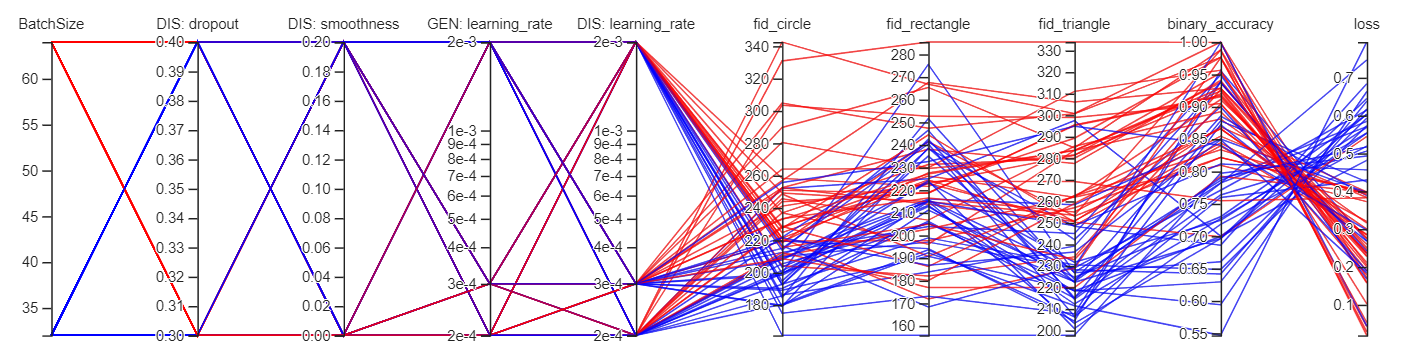
\includegraphics[width=0.75\textheight]{kapitel/5_ergebnisse/densegan/hyperparameter.PNG}
	\caption{Hyperparameter-Ansicht des Dense-GAN}
	\label{ergebnis:densegan-hyper}
\end{figure}

Auf der linken Seite sind alle Hyperparameter aufgelistet.
Die Abkürzung \textit{GEN} steht dabei für den Generator und \textit{DIS} repräsentiert den Diskriminator.
Außerdem können die einzelnen Graphen in einem Farbverlauf von Rot nach Blau einsortiert werden.
In der Abbildung \ref{ergebnis:densegan-hyper} wurde nach der BatchSize sortiert.

\subsection{Bilder}
Wie bereits beschrieben, werden neben den Hyperparameter und Metriken auch generierte Bilddaten protokolliert.
Neben den FID-Werten, kann so die generierten Ergebnisse subjektiv Bewerter werden.
Die subjektiv besten Figuren sind in der Abbildung \ref{ergebnis:densegan-good-example} zu sehen.
Die Figuren mit den besten FID-Werten werden in der Abbildung  \ref{ergebnis:densegan-best-fid} gezeigt.
Es lässt sich leicht erkennen, das die subjektive Bewertung und FID-Werte nicht übereinstimmen.

\todo{pack bilder nebneinander}
\begin{figure}[H]
	\centering
	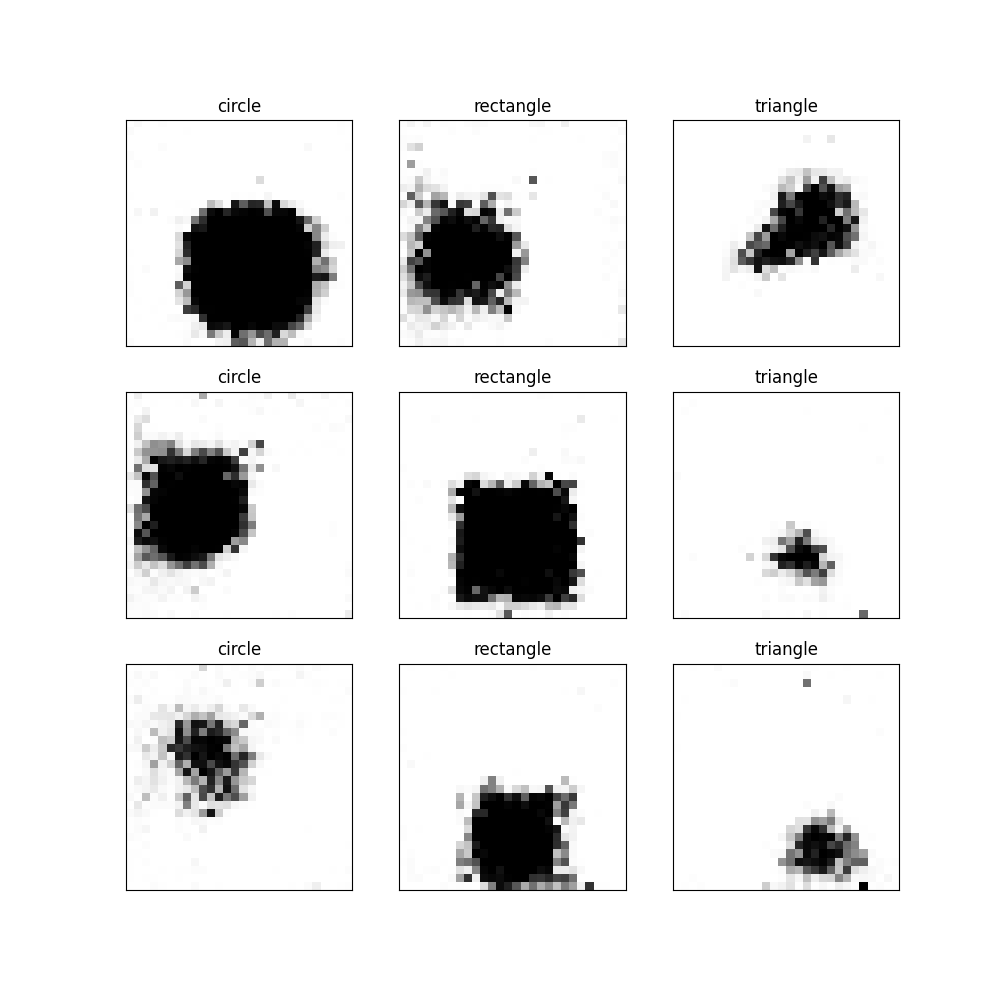
\includegraphics[height=0.4\textheight]{kapitel/5_ergebnisse/densegan/good_example.png}
	\caption{Gutes Beispiel des Dense-GAN}
	\label{ergebnis:densegan-good-example}
\end{figure}

\begin{figure}[H]
	\centering
	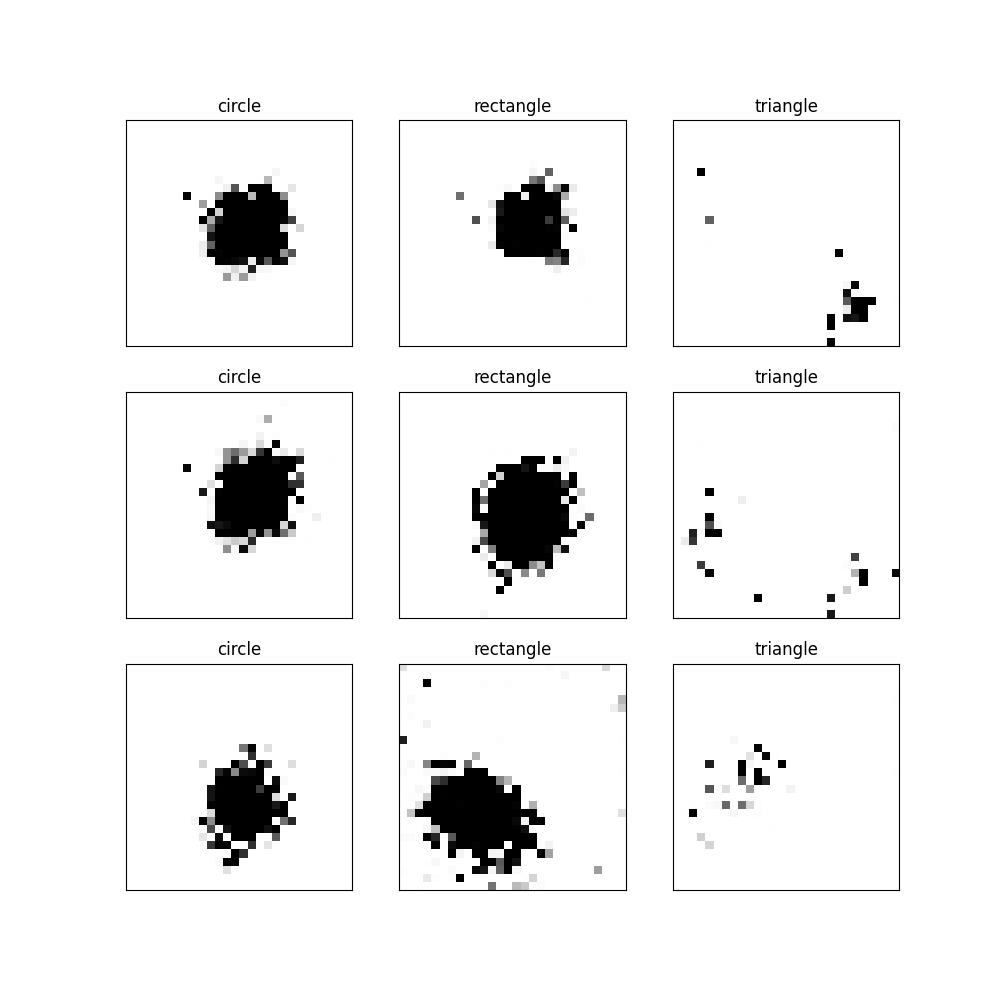
\includegraphics[height=0.4\textheight]{kapitel/5_ergebnisse/densegan/best_fid.png}
	\caption{Beste FID Werte des Dense-GAN}
	\label{ergebnis:densegan-best-fid}
\end{figure}

\subsection{Long Run}

\section{DC-GAN-Late-Label}
\begin{itemize}
	\item Tensorboard Graph -> beste Hyperparameter?
	\item 'beste' Bilder
\end{itemize}

\section{DC Generator und Dense Discriminator}

\section{Dense Generator und DC Discriminator}

\section{DC-GAN-Medical-Inspired}
\begin{itemize}
	\item Tensorboard grafik
	\item Beste Bilder
	\item Hyperparameter Analyse
\end{itemize}
